%%%%%%%%%%%%%%%%%%%%%%%%%%
%                          %
% ----- INTRODUCTION ----- %
%                          %
%%%%%%%%%%%%%%%%%%%%%%%%%%

\section{Introduction}

	\subsection{Idée}

		Le but recherché de l'outil est de sensibiliser les utilisateurs aux informations que ceux-ci dévoilent potentiellement en naviguant sur le web. Pour ce faire, nous avons besoin d'amasser des données sur leurs habitudes de navigation afin de les analyser.

		Ces données seront centralisées sur un serveur afin que nous puissions lancer des traitements sur l'ensemble des données plus tard dans le but de tenter de révéler des tendances, habitudes ou corrélations entre les données.

		De plus, nous souhaitons également offrir un service direct à l'utilisateur afin que celui-ci ait un bénéfice à installer l'extension et nous autoriser à accéder à ces données. Nous allons lui montrer via une interface web les données que nous avons pu amasser sur sa navigation depuis l'installation du plug-in, au travers de plusieurs pages et visualisations.

		Nous souhaitons également que les données récupérées ne puissent pas être utilisées pour reconnaître une personne particulière. C'est pourquoi le plug-in ne nécessite aucune connexion avec un compte externe, et ne demande pas information directement divulgatrice d'une identité.

		Nous pouvons ainsi résumer les caractéristiques principales du plug-in en quelques points.

		Le plug-in :
		\begin{itemize}
			\item Récupère les informations de navigation de l'utilisateur
			\item Envoie ces informations de manière anonyme à un serveur centralisé
			\item Propose une visualisation des données récoltées et calculées sur l'utilisateur
		\end{itemize}

	\subsection{Architecture}

		Le projet dans son ensemble requiert le développement d'un minimum de deux parties différentes :

		\begin{itemize}
			\item Une extension pour navigateur afin de récupérer et d'envoyer les données
			\item Un serveur recevant les données des extensions installées
		\end{itemize}

		Une troisième partie s'occupant de l'interface utilisateur est également à prévoir, celle-ci pouvant se situer autant dans l'extension que sur le serveur. La décision est finalement prise d'héberger l'interface utilisateur sur un différent serveur, auquel se connecte l'interface lorsque l'utilisateur souhaite accéder à sa page.

		\begin{figure}[h]
			\centering
			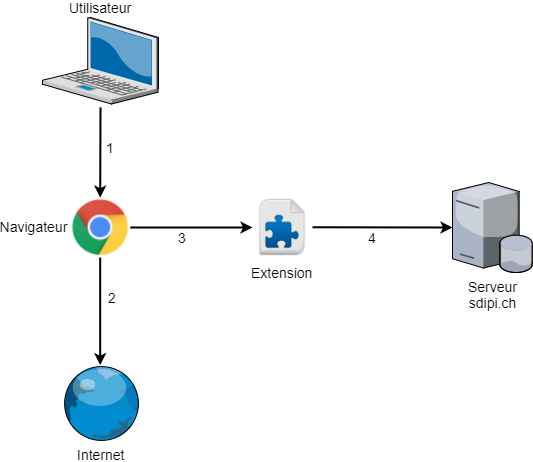
\includegraphics[width=0.8\textwidth]{images/design/intro/architecture}
			\caption{Flux de données de l'extension.}
			\label{d-architecture}
		\end{figure}

		La figure \ref{d-architecture} schématise la récolte de données effectuée par l'etension.
		\begin{enumerate}
			\item L'utilisateur entre une URL dans son navigateur
			\item Le navigateur accède à la ressource concernée
			\item Le navigateur transmet au plug-in les informations concernant la navigation
			\item Le plug-in contacte le serveur SDIPI pour lui transmettre les informations
		\end{enumerate}

	\subsection{Données}

		Les possibilités de récolte de données depuis une extension de navigateur sont extrêmement nombreuses. Nous allons cependant nous concentrer sur l'amassage de données utiles à l'étude, et qui ne représentent pas une menace à l'intimité de l'utilisateur. Nous devons donc nous limiter à un set de données adéquat. 

		Voici les différents types d'informations que nous récoltons, et à quelles fins chaque type d'information est utilisé :

		\subsubsection{Visite d'une URL}
			
			Lorsque l'utilisateur accèds à une nouvelle URL dans son navigateur, qu'il s'agisse d'un clic sur un lien ou d'une entrée dans la barre d'adresse, l'extension enregistre une partie de l'URL accédée ainsi que la date d'accès. Pour des raisons de protection de la vie privée, seule une partie de l'URL est conservée et envoyée au serveur.

			\begin{figure}[h]
				\centering
				$\underbrace{\texttt{https://www.google.ch/search}}_{\text{Partie conservée}}$\texttt{?q=Recherche+test}
				\caption{Exemple d'URL et traitement}
				\label{d-url}
			\end{figure}

			La figure~\ref{d-url} montre que tous les paramètres de la requête ne sont pas conservés. Seuls le protocole (\texttt{http} ou \texttt{https}), le nom de domaine, l'éventuel numéro de port ainsi que le chemin d'accès à la ressource sont conservés. Nous évitons ainsi la possibilité de stocker des informations sensibles comme le nom d'utilisateur, qui peut parfois se trouver dans cette partie de l'URL de certains sites web.

		\subsubsection{Activité sur une page}

			À tout moment, l'utilisateur a probablement plusieurs onglets ou plusieurs fenêtres de navigateur ouvertes. Nous souhaitons nous intéresser à quelle page est actuellement en train d'être parcourure par l'utilisateur. À cette fin, nous détectons les évènements sur la page web : Appui sur une touche, ou clic de souris par exemple. Dès lors qu'il se passe plus de 30 secondes sans aucun évènement de la part de l'utilisateur, nous estimons qu'il ne regarde plus activement la page. Ce temps passé à s'insétresser à chaque page est également envoyé au serveur central toutes les 30 secondes.

		\subsubsection{Requêtes du navigateur}

			Lorsque le navigateur accède à une page web ou à d'autres moments, le navigateur doit charger des ressources qui se trouvent sur un serveur distant. Ce chargement peut prendre place pour afficher par exemple une image, un morceau de la page web elle-même, ou être demandé par un script chargé.

			Pour chaque requête que le navigateur envoie, l'extension mémorise certaines informations : 
			\begin{description}
				\item[Origine] L'extension mémorise l'URL de la page qui demande la ressource. Cette information est traitée de la même manière que décrit à la figure~\ref{d-url}.
				\item[Hôte] Toujours d'une manière identique à la figure~\ref{d-url}, l'extension mémorise également le serveur contacté.
				\item[Taille] L'extension mémorise également la taille de la requête en question, qui correspond à l'addition du contenu envoyé dans le contenu de celle-ci, ainsi que la taille des paramètres (ceux qui ne sont pas retenus par l'extension).
			\end{description}

		\subsubsection{Identificateur}

			Lors de l'installation de l'extension, un nombre aléatoire est généré pour l'installation. Cet identificateur est envoyé envoyé au serveur central en plus de chaque autre information : Elle nous est utile pour assigner chaque donnée de navigation avec un navigateur particulier.

\section{Extension}

	

\section{Serveur}



\section{Interface}

	